\documentclass[a4paper, 11pt]{article}
\usepackage{geometry}
\geometry{letterpaper, margin=1in}
\usepackage{amsmath}
\usepackage{amssymb}  
\usepackage{amsthm}
\usepackage{ulem} 
\usepackage{graphicx}
\usepackage{enumitem} 
\graphicspath{ {images/} }

\begin{document}
%Header-Make sure you update this information!!!!
\noindent
\large\textbf{Theorema Egregium} \hfill \textbf{John Waczak} \\
\normalsize MTH 435 \hfill  Date: \today \\
Dr. Christine Escher \\

	
\subsection*{(1)}
	\textit{Show that that if $\sigma$ is an orthogonal parametrization, that is $F=0$, then}
		\begin{equation}
			K = -\frac{1}{2\sqrt{EG}} \Bigg\{\Big(\frac{E_v}{\sqrt{EG}}\Big)_v + \Big(\frac{G_v}{\sqrt{EG}}\Big)_u\Bigg\}
		\end{equation}
	
	\begin{proof}
		To prove equation (1) holds I will first simplify the equation as much as possible and then will show that the general curvature equation derived from the Christoffel symbols (5.11) reduces to this formula when we set $F=0$. 
			\begin{align}
				\partial_v \Big(E_v(EG)^{-1/2}\Big) &= \frac{E_{vv}}{\sqrt{EG}}-\frac{1}{2}\frac{E_vE_vG}{(EG)^{3/2}} - \frac{1}{2}\frac{E_vG_vE}{(EG)^{3/2}} \nonumber\\ 
				\partial_u \Big( G_u(EG)^{-1/2} \Big) &= \frac{G_{uu}}{\sqrt{EG}}-\frac{1}{2}\frac{G_uE_uG}{(EG)^{3/2}}-\frac{1}{2}\frac{G_uG_uE}{(EG)^{3/2}} \nonumber \\ 
				\Rightarrow K &= \frac{-\frac{1}{2}E_{vv}EG+\frac{1}{4}E_vE_vG+\frac{1}{4}E_vG_vE-\frac{1}{2}G_{uu}EG+\frac{1}{4}G_uE_uG+\frac{1}{4}G_uG_uE}{(EG)^2}
			\end{align}
		\noindent Now we start with equation (5.11) from the text substituting $F=0$. 
			\begin{align}
				K &= \frac{\begin{vmatrix}
						-\frac{1}{2}E_{vv} & -\frac{1}{2}G_{uu} & -\frac{1}{2}E_v \\
						-\frac{1}{2}G_u & E & 0 \\ 
						\frac{1}{2}G_v & 0 & G
					\end{vmatrix} -\begin{vmatrix}
						0 & \frac{1}{2}E_v & \frac{1}{2}G_u \\ 
						\frac{1}{2}E_v & E & 0 \\ 
						\frac{1}{2}G_u & 0 & G 
					\end{vmatrix}}{(EG)^2} \nonumber \\ 
				&= \frac{(-\frac{1}{2}E_{vv}-\frac{1}{2}G_{uu})EG-(\frac{1}{2}E_u)(-\frac{1}{2}G_uG)+\frac{1}{2}E_v\frac{1}{2}G_vE-(-\frac{1}{2}E_v\frac{1}{2}E_vG+\frac{1}{2}G_u(-\frac{1}{2}G_uE)}{(EG)^2} \nonumber \\ 
				&= \frac{-\frac{1}{2}E_{vv}EG-\frac{1}{2}G_{uu}EG+\frac{1}{4}E_uG_uG+\frac{1}{4}E_vG_vE + \frac{1}{4}E_vE_vG+\frac{1}{4}G_uG_uE}{(EG)^2} 
			\end{align}
		Equivalence follows from equations (2) and (3). Thus, equation (1) holds for the curvature when $F=0$. 
	\end{proof}
	
\subsection*{(2)}
	\textit{Verify that the surfaces
			\begin{align*}
				\sigma(u,v) &= (u\cos v, u\sin v, \ln u) \\ 
				\tilde{\sigma}(u,v) &= (u\cos v, u\sin v, v) 
			\end{align*}
	have equal Gaussian curvature at all points but the map $\tilde{\sigma}\circ\sigma^{-1}$ is not an isometry. Use a mathematical software package to graph the surfaces.}

	\begin{proof}
		First I will compute the Gaussian curvatures to show that they are the same. Note that these surfaces are the helicoid and catenoid which we already showed to have the same Gaussian curvature in a previous exercise. Now that we have an intrinsic definition for $K$ though, I will try and use one of these new definitions instead. First we need $E, F, G, \tilde{E}, \tilde{F}, \tilde{G}$. 
			\begin{align*}
				\sigma_u &= (\cos v, \sin v, \frac{1}{u}) \\ 
				\sigma_v &= (-u\sin v, u\cos v, 0)\\ 
				\tilde{\sigma}_u &= (\cos v, \sin v, 0 ) \\ 
				\tilde{\sigma}_v &= (-u\sin v, u\cos v, 1) \\ 
				E &= 1 + \frac{1}{u^2} \\ 
				F &= 0 \\ 
				G &= u^2 \\
				\tilde{E} &= 1 \\ 
				\tilde{F} &= 0 \\ 
				\tilde{G} &= u^2 + 1
			\end{align*}
		\noindent Observe that both $F=0$ and $\tilde{F} =0$. This means that we can use the result from problem 1 to quickly calculate the curvatures of both surfaces. 
			\begin{align}
				E_v &= 0, \quad G_u = 2u, \quad EG = u^2 + 1 \nonumber\\ 
				\Rightarrow K &= -\frac{1}{2\sqrt{u^2+1}}\Bigg(\frac{2u}{\sqrt{u^2+1}}\Bigg)_u \\ 
				\tilde{E_v} &= 0, \quad \tilde{G_u} = 2u, \quad EG = u^2+1 \nonumber\\ 
				\Rightarrow \tilde{K} &= -\frac{1}{2\sqrt{u^2+1}}\Bigg(\frac{2u}{\sqrt{u^2+1}}\Bigg)_u
			\end{align}
		\noindent Thus we have that the Gaussian curvatures are equal for all points. Now we must show that $f=\tilde{\sigma}\circ\sigma^{-1}$ is not an isometry. Recall from exercise 3.101 from last term that a diffeomorphism $f$ is an isometry if and only if $f\circ\sigma$ preserves the first fundamental form. Observe that $f\circ\sigma = \tilde{\sigma}\circ\sigma^{-1}\circ\sigma=\tilde{\sigma}\circ\text{Id} = \tilde{\sigma}$. Thus we have that $f$ is an isometry if and only if $\tilde{sigma}$ has the same first fundamental form as $\sigma$. This can not be true as $E\neq\tilde{E}$ and $G\neq\tilde{G}$. Thus $\sigma, \tilde{\sigma}$ share the same Gaussian curvature but are not isometric. 
			\begin{figure}[!hbt]
				\centering
				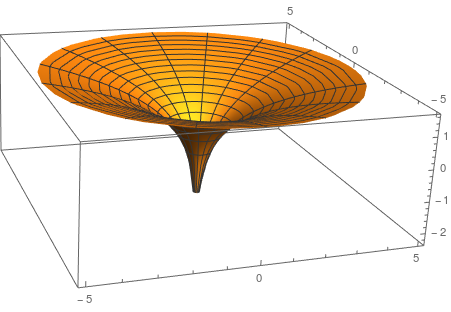
\includegraphics[width=0.4\columnwidth]{Catenoid}
				\caption{$\sigma = (u\cos v, u\sin v, \ln u )$, the catenoid}
			\end{figure}
			\begin{figure}[!hbt]
				\centering
				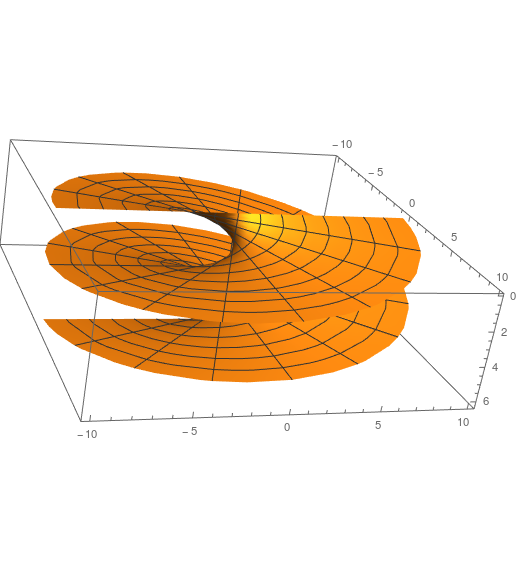
\includegraphics[width=0.4\columnwidth]{Helicoid}
				\caption{$\tilde{\sigma}=(u\cos v, u\sin v, v)$, the helicoid}
			\end{figure}	
	\end{proof}
	
\subsection*{(3)}
	\textit{Show that there exists no surface with $\sigma(u,v)$ such that $E=G=1$, $F=0$, and $e=1$, $g=-1$, and $f=0$.} 
	
	\begin{proof}
		To prove the above statement, we will calculate the curvature using two different methods in order to show a contradiction. Thus, assume $\exists$ a surface $\sigma(u,v)$ such that the surface has $E,F,G,e,f,g$ given in the problem statement. Since we have that $F=0$ and $E=1$, Corollary 5.55 gives that 
			\begin{align}
				K &= \frac{-\sqrt{G}_{uu}}{\sqrt{G}} = \frac{-0}{1} = 0
			\end{align}
		As $G$ is a constant function and therefore has $0$-valued partial derivatives of all orders. Now recall our original \textit{extrinsic} definition of the Gaussian curvature that employed $e,f,g$. 
			\begin{align}
				K &= \frac{eg-f^2}{EG-F^2} = \frac{-1-0}{1-0} = -1 
			\end{align}
		Thus, equations (6) and (7) give us a contradiction. Therefore we conclude that there is no surface satisfying $E=G=1$, $F=0$, $e=1$, $g=-1$, and $f=0$. 
	\end{proof}
	
	
	
\subsection*{(4)}
	\textit{Compute the Christoffel symbols for an open set of the plane \begin{enumerate}[label=(\alph*)]
			\item In Cartesian coordinates 
			\item In Polar coordinates 
		\end{enumerate}
	Use the Gauss formula to calculate K in both cases}\\ 
	
	\begin{proof}[(a)]
		First, consider the following parametrization of the plane: $\sigma(u,v)=(u,v,0)$. From this we can derive the following:
			\begin{align*}
				\sigma_u(u,v)&= (1,0,0) \\ 
				\sigma_v(u,v)&= (0,1,0) \\ 
				\Rightarrow \sigma_{uu} &= \sigma_{uv} = \sigma_{vv} = (0,0,0) \\ 
			\end{align*} 
		Since the Christoffel symbols $\Gamma_{ij}^k$ are the coefficients in the expansion of the second partial derivatives of our chart in the $\{\sigma_u, \sigma_v, N\}$ frame we have that $\Gamma_{ij}^k = 0 \quad \forall i,j,k\in\{1,2\}$. Thus from the Gauss formula for the curvature, we conclude that the curvature of the plane is 0 (as expected). 
	\end{proof}
	
	\begin{proof}[(b)]
		For polar coordinates, we have the following map. $\sigma(r,\theta) =(r\cos\theta, r\sin\theta, 0)$. This leads to the following:
			\begin{align*}
				\sigma_r(r,\theta) &= (\cos\theta, \sin\theta, 0) \\ 
				\sigma_\theta(r,\theta) &= (-r\sin\theta, r\cos\theta, 0) \\ 
				\Rightarrow E&= 1, \quad F=0, \quad G=r^2 \\ 
			\end{align*}
		Now that we have $E,F,G$ we can compute the Christoffel symbols from Proposition 5.53. Note that $\alpha = 2EG-2F^2=2r^2$. Thus, 
			\begin{align*} 
				\text{(a)} \quad \Gamma_{11}^1 &= 0 &\Gamma_{11}^2 &= 0\\ 
				\text{(b)} \quad \Gamma_{12}^1 &= 0 &\Gamma_{12}^2 &= \frac{1}{r} \\
				\text{(c)} \quad \Gamma_{22}^1 &= -r &\Gamma_{22}^2 &= 0
			\end{align*}
		Now using Gauss's Formula (1v) the Gaussian curvature is:	
			\begin{align*}
				EK &= (\Gamma_{11}^2)_v - (\Gamma_{12}^2)+\Gamma_{11}^1\Gamma_{12}^2+\Gamma_{11}^2\Gamma_{22}^2-\Gamma_{12}^1\Gamma_{11}^2-(\Gamma_{12}^2)^2 \\ 
				\Rightarrow K&= -\Big(\frac{1}{r}\Big)_r -\Big(\frac{1}{r}\Big)^2 \\ 
					&= -\Big(-\frac{1}{r^2}\Big)-\frac{1}{r^2} = 0
			\end{align*}
		Hooray, the Gaussian curvature remained independent of our choice of surface chart when we using Gauss's Formula to calculate the curvature! 
	\end{proof}
	
	
	
\subsection*{(5)}
	\textit{Justify why the surfaces listed below are not pairwise locally isometric\begin{enumerate}[label=(\alph*)]
			\item Sphere
			\item Cylinder
			\item Saddle Surface $z = x^2-y^2$
		\end{enumerate}}
	\begin{proof}
		To prove that these surfaces are not pairwise locally isometric, we will use the contrapositive of Gauss's Theorema Egregium: if $\exists p\in S$ such that $K(p)\neq K(f(p))$ then $f:S\rightarrow\tilde{S}$ is not an isometry between the surfaces. If we can show that the curvatures are constants that disagree, then the contrapositive would be true for any function and thus there can be no isometry between the surfaces. That being said, let's calculate the curvatures for the three surfaces. Define the following surface patches for the three cases:
			\begin{align*}
				\sigma^s(u,v) &= (\sin v \cos u, \sin v \sin u, \cos v) \\ 
				\sigma^c(u,v) &= (\cos u, \sin u, v) \\ 
				\sigma^g(u,v) &= (u, v, u^2-v^2) 
			\end{align*} 
		First lets work with the sphere $\sigma_s$. 
			\begin{align*}
				\sigma_u^s(u,v) &= (-\sin v\sin u, \sin v \cos u, 0) \\ 
				\sigma_v^s(u,v) &= (\cos v \cos u, \cos v \sin u, -\sin v) \\ 
				E^s &= \sin^2 v \\ 
				F^s &= 0 \\ 
				G^s &= 1
			\end{align*} 
		Since $F$ is zero, we can again use the the formula from the first problem. 
			\begin{align*}
				E^s_v &= 2\sin v \cos v, \quad G^s_u = 0 \\ 
				K^s &= -\frac{1}{\sqrt{\sin^2v}}\Big(\frac{\sin v\cos v}{\sqrt{\sin^2 v}}\Big)_v \\ 
					&= -\frac{1}{\sin v}\Big(\cos v\Big)_v = \frac{\sin v}{\sin v} = 1
			\end{align*}
		This is as expected. Now let's show that the cylinder has 0 curvature (if you look closely it's just the plane anyway). 
			\begin{align*}
				\sigma_u^c(u,v) &= (-\sin u, \cos u, 0) \\ 
				\sigma_v^c(u,v) &= (0, 0, 1) \\ 
				E^c &= 1 \\ 
				F^c &= 0 \\ 
				G^c &= 1 \\ 
				E_v^c &= 0 \\ 
				G_u^c &= 0 \\ 
			\end{align*}
		Again we have $F=0$ but we also have that $	E_v^c = 0$ and $G_u^c = 0$ which implies via the equation from problem one that the Gaussian curvature is $K^c=0$ as expected. Now let's determine the curvature of the saddle surface. To make our live's easier, recall Example 4.18 which states that for a graph $\phi(x,y)$ the Gaussian curvature is $K = \frac{\phi_{xx}\phi_{yy}-\phi^2_{x,y}}{(1+\phi_x^2+\phi_y^2)^2}$. 
			\begin{align*}
			 \phi(u,v) &= u^2 - v^2 \\ 
			 \phi_u &= 2u \\ 
			 \phi_v &= -2v \\ 
			 \phi_{uu} &= 2 \\ 
			 \phi_{uv} &= 0 \\ 
			 \phi_{vv} &= -2 \\ 
			 \Rightarrow K^g &= \frac{-4}{(1+4u^2+4v^2)^2}
			\end{align*}
	
	\noindent Thus we have shown that the sphere and cylinder both have different constant curvatures and the saddle surface has a position dependent curvature. Thus there can be no isometry between these surfaces. To be a little more precise, for the case of y cylinder and the sphere we have that for all points the curvature differs and so there can't be any isometry because this would be true independent of $f$. For the saddle surface we are comparing a curvature that depends on position to constant curvatures and so we easily have that because the curvature of a surface is independent of chart, for any function f that maps one surface to the other we will have one if not more points where the curvatures disagree. 
	\end{proof}
	

	
	
	
	
	
	
	
	
	
	
	
	
	
	
	
	
	
	
	
	
	
	
	
	
	
	
	
	
	
\end{document}